\chapter{Amazon Web Services}\label{chapter:kapitellabel} %%%%%%%%%%%%%%%%%%%%%%%%%%%%
Amazon Web Services (AWS) gehört zum amerikanischen Online-Versandhändler Amazon und beschreibt die
seit 2006 entwickelten Infrastrukturdienstleistungen, welche zu Beginn für andere Unternehmen angeboten
wurden und seit {{\color{red}2012 im Zuge der voranschreitenden Cloud-Computing-Technologie auch
privaten Nutzern angeboten werden} \cite{aws:general}. Ihren Ursprung haben die Dienste in den Versuchen Amazon's, Kosten einzusparen. Als Online-Versandhändler unterliegt das Unternehmen einem dynamischen
Nutzungsaufkommen. Gerade zu saisonalen Ereignissen wie Weihnachten sind die Anfragen
an die Webseiten und damit an die bereitgestellten IT-Ressourcen gut zehnmal höher als
in der restlichen Zeit des Jahres. Damit die Ressourcen in dieser Zeit nicht ungenutzt
bleiben und nur Geld kosten, entstand die Idee, die freien Kapazitäten an Dritte zu verkaufen.
Dabei nutzt Amazon den Pooling-Effekt: Ungenutzte Ressourcen landen in einem gedachten Pool und
können je nach Bedarf weitergenutzt werden. Hierdurch gelingt es Amazon ein für Nutzer
sehr attraktives Modell zu schaffen, durch welches sie sich je nach Bedarf flexible
Ressourcen und Kapazitäten zusammenstellen können \cite{baun:cloudcomp}.

AWS ist eine öffentliche Cloud (weitere Cloudtypen vgl. \cite{wittig:awsinaction}, \cite{baun:cloudcomp}). Das bedeutet, sie wird durch eine Organisation verwaltet und steht der Öffentlichkeit zur Verfügung. Mit seinem Angebot deckt AWS folgende Klassifizierungen für Cloud Computing Dienste ab.
\begin{enumerate}
  \item Infrastructure as a Service (IaaS)
  \\AWS bietet grundlegende Ressourcen wie Berechnung (computing), Speicherung (storage) und Netzwerk Kapazitäten (network capabilities). Ein Kerndienst hierfür ist Elastic Compute Cloud (EC2). Weitere sind Dynamo, S3, SimpleDB, CloudFront und SQS.
  \item Platform as a Service (PaaS)
  \\AWS bietet beispielsweise über Elastic Beanstalk eine Plattform, über welche kundenspezifische Anwendungen in der Cloud bereitgestellt werden können.
  \item Software as a Service (SaaS)
  \\SaaS kombiniert die vorhandene Infrastruktur mit der verfügbaren Software in der Cloud. Dies bietet AWS zum Beispiel mit dem Dienst Workspaces, welcher es ermöglicht, über seinen Desktop in der Cloud zu verfügen.
  \item Humans as a Service (HuaaS)
  \\ Hierbei geht es um Dienste, bei denen der Mensch als Ressource ins Spiel kommt, da dieser der Maschine in einigen Bereichen deutlich überlegen ist. Zum Beispiel in Übersetzungs- oder Design-Aufgaben. Bei Amazon Mechanical Turk übernimmt eine Gruppe von Menschen Aufgaben unterschiedlicher Größe und Komplexität und erhält dafür je Kopf eine entsprechende Entlohnung. Damit entspricht der Dienst einem Marktplatz für CrowdSourcing-Angebote.
\end{enumerate} \cite{wittig:awsinaction}, \cite{baun:cloudcomp}

Amazon dominiert den Markt im Bereich SaaS deutlich (45 Prozent Marktanteil), was sich auch in den Umsatzzahlen zeigt. Im dritten Quartal 2016 konnte AWS ein Umsatzplus von 55 Prozent auf 3,2 Milliaren US-Dollar für sich verbuchen. Das macht mittlerweile etwa 10 Prozent des Gesamtumsatzes von Amazon aus. \cite{t3n:brien}

Die, über AWS, bereitgestellten Dienste können grob in nachfolgende Gruppen unterteilt werden. Dabei beschränkt sich die Liste auf die wesentlichen der aktuell über 50 verfügbaren Dienste \cite{sendcheckit:plain}.

\begin{itemize}
  \item Berechnungs-Dienste
  \\ Beinhaltet die Bereitstellung von Rechenleistung und Speicherplatz z.B. Virtuelle Server.
  \item Applikations-Dienste
  \\ Diese Dienste bieten Lösungen für allgemeine Anwendungsfälle z.B. Queueing oder das Durchsuchen großer Datenmengen.
  \item Dienste für das Unternehmen
  \\ Hiermit sind unahängige Dienste wie z.B. Mail Server oder Directory Services gemeint.
  \item Entwicklungs- und Administrations-Dienste
  \\ Diese Dienste basieren auf den bereits oben genannten Diensten und sind hilfreich bei Themen wie Zugangsberechtigungen vergeben und einrichten, virtuelle Server monitoren und dem Bereitstellen von Anwendungen.
  \item Speicher
  \\ Hierbei wird das Sammeln, Persistieren und Archivieren von Daten betrachtet.
  \item Datenbank-Speicher
  \\ Die genannten Dienste bieten gegenüber der "´einfachen"' Speicheroption einige Vorteile, wenn es ums Managen strukturierter Daten geht. Es werden relationale und NoSQL-Systeme untersützt.
  \item Netzwerk
  \\ Die letzte Gruppe Netzwerk beinhaltet Dienste, die es zum Beispiel ermöglichen private Netzwerke zu definieren oder ein Domain Name System (DNS) für seine Anwendung einzurichten.
\end{itemize} \cite{wittig:awsinaction}

Amazon betreibt und verwaltet
die über ein Netzwerk miteinander verbundene Hardware, welche für die korrekte
Funktion der Anwendungsservices benötigt wird, sowie die benötigten Ressourcen,
welche über eine Webanwendung bereitgestellt und genutzt werden. Mit seinem Angebot
zählt AWS zu den bedeutendsten internationalen Angeboten im Cloud Computing.

\section{Regionen und Availability Zones}
AWS verfügt derzeit über 42 Availability Zones (Verfügbarkeitszonen) in 16 geografischen Regionen weltweit verteilt. Verschiedene Dienste, darunter EC2 und S3, sind in Regionen eingeordnet.

\begin{figure}[!ht]
  \centering
  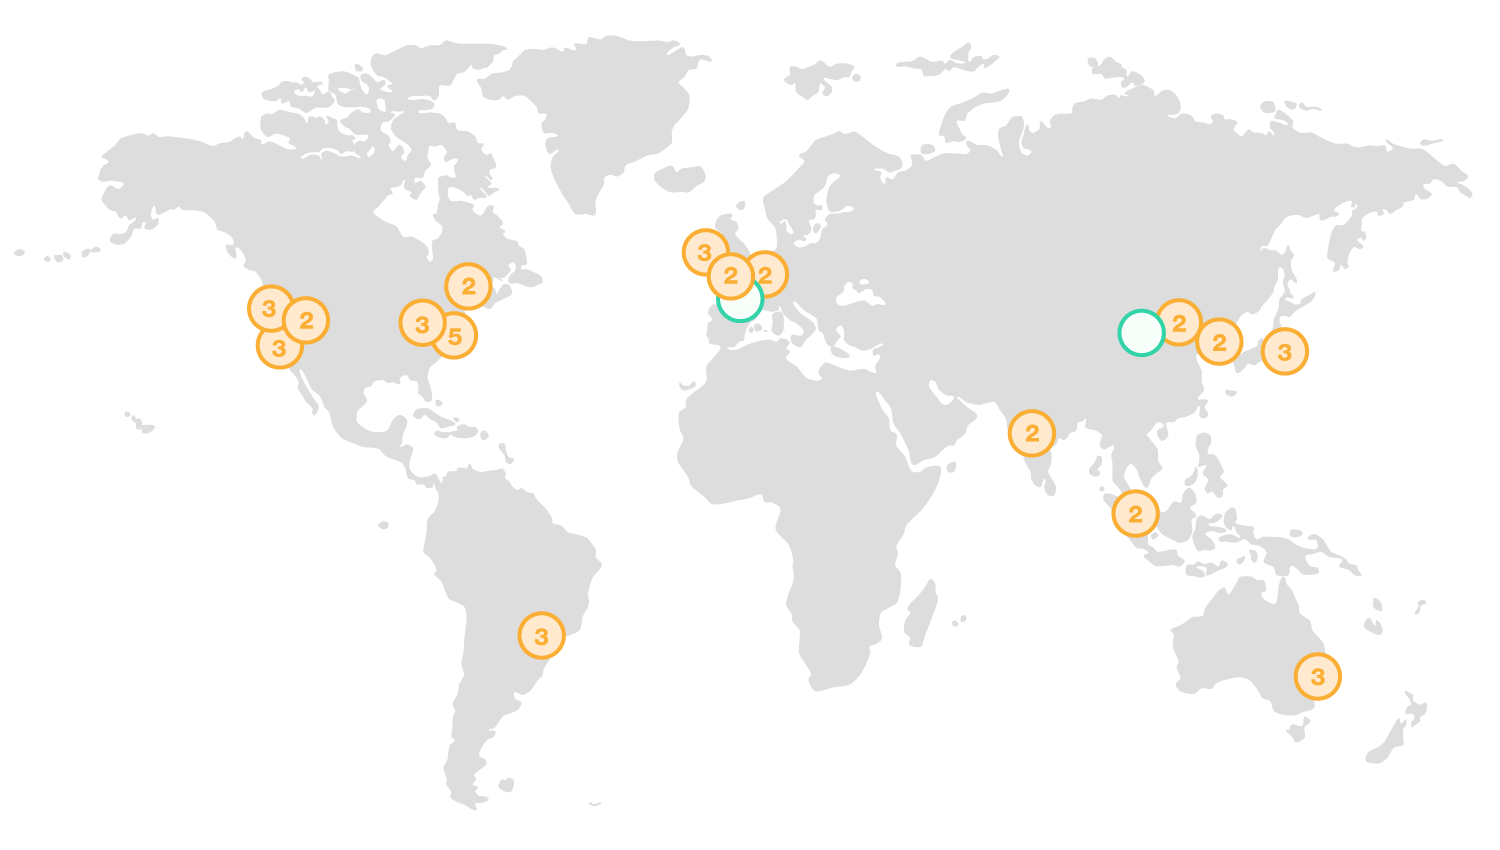
\includegraphics[width=0.9\textwidth]{images/regions.png}
  \caption{weltweite Infrastruktur (orange: Region mit x AZs, weiß/grün: geplante Region) \cite{aws:regions}}
\end{figure}

Eine Region entspricht einem physischen Ort auf der Welt, welcher mehrere Availability Zones (AZs) beherbergen kann. Bei einer AZ handelt es sich um ein oder mehrere unabhängige Rechenzentren, wobei jedes eine redundante Energieversorung, Netzwerk und Konnektivität besitzt (siehe \ref{figure:azs-regions}).

\begin{figure}[!ht]
  \centering
  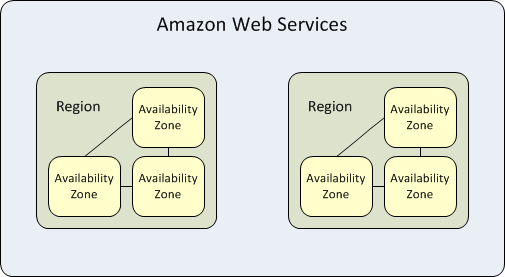
\includegraphics[width=0.7\textwidth]{images/azs_regions.png}
  \caption{Regionen mit zugehörigen Availability Zones \cite{aws:azs}}\label{figure:azs-regions}
\end{figure}

Dies erhöht die Ausfallsicherheit im Falle physischer Schäden z.B. Stürme und ist ein Alleinstellungsmerkmal gegenüber fast allen anderen Anbietern für technologische Infrastrukturen. Es ist daneben auch möglich, Daten zwischen mehreren AZs auszutauschen, um dem Ausfall der Anwendung bei einem Ausfall von AZs in einer Region vorzubeugen. Die AZs sind dafür mit schnellen, privaten Glasfasernetzwerken verbunden.
Durch die Replikation der Daten über mehrere geografische Regionen hinweg, kann die Redundanz und Fehlertoleranz noch zusätzlich erhöht werden.

Die weltweit verteilten Datenzentren sind gerade für international agierende Unternehmen interessant. Je näher ein Datenzentrum dem Endkunden einer Anwendung ist, welche bei AWS gehostet wird, desto geringer fallen die Latenzzeiten aus. Darüberhinaus punktet Amazon mit diesem Konzept beim Thema Datenschutz. In Frankfurt am Main sind 2014 zwei AZs entstanden um Bedenken deutscher Unternehmen hinsichtlich Datenschutz auszuräumen. Kunden können definieren, dass ihre Daten ausschließlich in deutschen Rechenzentren gehalten und bearbeitet werden. Damit unterliegen die dort gehosteten Daten den deutschen Datenschutz-Vorgaben.

Aktuell sind fünf weitere Availability Zones und zwei weitere Regionen geplant.
\\ \cite{computerwoche:reder}, \cite{aws:regions}, \cite{aws:azs}

\section{Vorteile}
\section{Kosten}
\section{Sicherheit}

% keep an blank line above
